\documentclass[10pt,letterpaper]{amsart}
\usepackage[T1]{fontenc}
\usepackage[utf8]{inputenc}
\usepackage[american]{babel}
\usepackage{lmodern}
\usepackage{amsfonts,amsmath}
\usepackage[left=25mm,right=25mm,top=38mm,bottom=34mm]{geometry}
\usepackage{microtype}
\usepackage{graphicx}
\usepackage{booktabs}
\usepackage{tabularx}
\usepackage{caption}
\usepackage{placeins}
\usepackage[numbers,sort&compress]{natbib}
\usepackage[hidelinks]{hyperref}

\input{glyphtounicode}
\pdfgentounicode=1
\hypersetup{
  pdftitle={Information Retention in Chains of Language Model Agents},
  pdfauthor={Marco D'Addezio},
  pdfsubject={A ten-hop experiment on summarization, incoming information, and source access}
}
\graphicspath{{figures/}}
\urlstyle{same}
\captionsetup{font=small,labelfont=bf,labelsep=period,skip=6pt}
\captionsetup[table]{position=top}

\linespread{1.05}
\setlength{\parindent}{0pt}
\setlength{\parskip}{0.45em plus 0.12em minus 0.08em}
\setlength{\textfloatsep}{14pt plus 3pt minus 3pt}
\setlength{\intextsep}{10pt plus 2pt minus 2pt}
\renewcommand{\arraystretch}{1.19}
\renewcommand{\topfraction}{0.85}
\renewcommand{\bottomfraction}{0.75}
\renewcommand{\textfraction}{0.12}
\setlength{\emergencystretch}{1em}
\clubpenalty=10000
\widowpenalty=10000
\raggedbottom
\setcounter{tocdepth}{1}
\numberwithin{equation}{section}

\begin{document}

\title[Information retention in agent chains]{Information Retention in Chains of Language Model Agents}
\author{Marco D'Addezio}
\date{20 November 2026}
\keywords{Language model agent, information retention, repeated summarization, beta-geometric decay, cure model}

\begin{abstract}
How much factual information survives when language model agents hand off short notes
and new information arrives between handoffs? We analyze 960 ten-relay chains for
80 synthetic business documents. Claude Haiku subagents in Claude Code handled relay
requests in shared batches. Each relay was asked for at most 67 words. From the second
relay onward, it received the previous note and a new paragraph. We varied renewed
access to the original document and an instruction to preserve specifics. Without
renewed source access, the instruction improved measured retention of original facts
at the first two relays. The effect reversed at relay three. By relay ten, 9.4\% of
original facts were scored correct under the baseline and 1.6\% under the instruction.
Notes under the instruction retained more incoming facts per word. With source access,
the pooled endpoint rates were 25.2\% and 27.9\%. The endpoint differences varied across
replicates. A model that separates first inclusion from later retention best predicted
incoming-fact correctness for held-out documents within this run. One reviewer agreed
with both scorers on 93 original-fact judgments across five notes, including 85 omissions.
The spot check contained no within-document prompt pairs. The results describe this
batched run, with repeatability in fresh execution contexts still open.
\end{abstract}
\maketitle

{\small\tableofcontents}

\section{Introduction}
\label{sec:introduction}

How much information is lost when one language model agent hands its work to the next?
Consider a workflow in which each agent passes forward a short note so that the next can
continue the task. The note determines which details remain available from the preceding
step. It might give the day and month of a deadline and omit the year. It might report a
4\% late-delivery penalty without saying how late a delivery must be to trigger it. Either
change can affect what the next agent understands or does.

Even a handoff that preserves most of its input can leave little of the original material
after repeated compression. If each step preserved 90\% of the still-present original
facts and omitted facts never reappeared, the expected share remaining after ten steps
would be $0.9^{10}\approx 35\%$. A constant rate is only a starting point. Some facts may
be easier to carry forward than others. When new information arrives, each agent also
has to decide which parts of the previous note to retain and which new facts to include.
If agents can reread the source, a fact omitted at one step can appear again at the next.
The question is therefore both how much survives each handoff and which facts remain
available over the life of a chain.

Prior work has used transmission chains to study changes in text properties such as
toxicity and readability across repeated language model rewrites~\cite{perezEtAl2025}.
Liu studies how much an agent's successor can learn from a written handoff in tasks
with hidden rules, including variants where notes are written from the full
record~\cite{yiboLiu2026Handover}. Our setting starts from known facts and adds new ones
at each later relay. It measures which details survive when we vary both access to the
original document and the instruction to preserve specifics.

We study these questions using 80 synthetic business documents with tracked facts such
as people, dates, codes, quantities, negations and conditional rules. At the first relay,
an agent sees the original document and is asked to write a note of at most 67 words.
At each subsequent relay, another agent sees the previous note and a new paragraph
describing a workstream. In condition~A, only the first agent sees the original
document. In condition~B, every agent can reread it. Within each condition we compare
the baseline prompt with an instruction to preserve specifics exactly. The resulting
960 chains let us follow original facts from the first compression onward and compare
incoming facts at the same number of relays since their introduction. Claude Haiku
subagents generated the notes in Claude Code. Each subagent answered a batch of requests
in a shared context, and outcomes can depend on that execution arrangement.

We measure retention as the share of tracked claims scored correct in the current note.
For a conditional rule, the claim includes both the circumstances that trigger it and
its consequence. This measure provides a way to compare notes of similar length even
when they carry different details. It covers the facts selected for tracking. We also
distinguish presence at a given relay from uninterrupted retention, since access to the
original document can allow a fact to reappear after an omission.

Figure~\ref{fig:original-retention} shows how quickly scored retention declines in the
recorded notes. In condition~A under the baseline prompt, 55.2\% of original facts
are scored correct after one relay, 26.6\% after three, and 9.4\% after ten. The
preservation instruction raises first-relay correctness to 62.4\%, but by the third
relay its advantage has reversed. By the tenth, the notes with that instruction contain
fewer original facts and more incoming facts per word. This pattern is consistent with
new details displacing original ones within the note. When agents can reread the
original document, the preservation instruction is associated with a small increase
in pooled original-fact correctness at the endpoint. Both endpoint differences vary
across the three replicates.

The analysis compares several descriptions of retention over time, including constant
decay, a distinct first relay, and models that account for a slowing decline. It also
examines how batch execution and the measurement process affect interpretation. The
human spot check tests agreement on a small set of existing notes. The experiment
estimates factual retention under a specific way of passing and updating short notes,
with separate evidence needed for other prompts, models or execution settings.

\begin{figure}[!htbp]
  \centering
  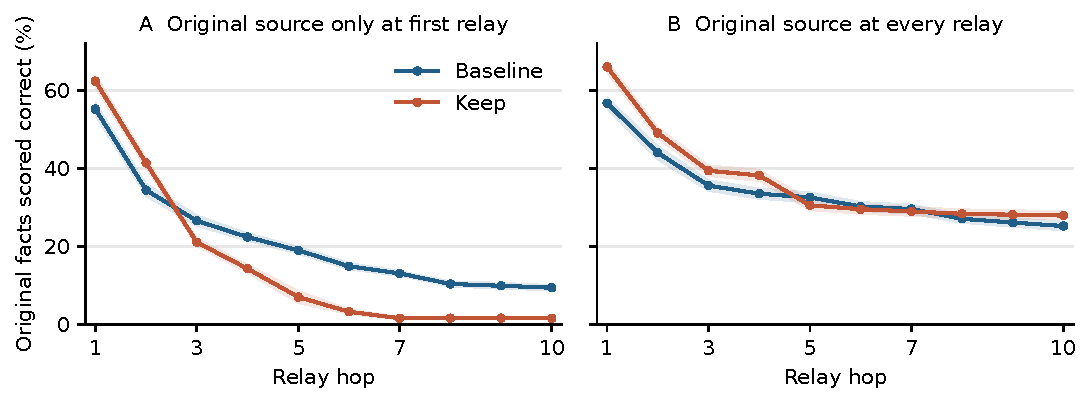
\includegraphics[width=\linewidth]{01_original_retention.pdf}
  \caption{Original facts scored correct across ten hops. Bands are pointwise 95\% document-bootstrap
    intervals over 20,000 draws. They condition on the recorded subagent executions and
    machine measurements; they do not include fresh-execution or human-validation uncertainty.}
  \label{fig:original-retention}
\end{figure}

\subsection*{Acknowledgments}

The author thanks Yacine Touati for asking the question that motivated this experiment.
The author received support from Anthropic through the Claude Team plan for scientists.

\subsection*{AI disclosure}

The main Claude Code session implemented and orchestrated the experiment; Haiku authored
notes and Sonnet supplied model measurements. Templates, reference values, span, unit and
parameter checks, aggregation and optimization were deterministic. Classification depended
on model-extracted answers and, for semantic facts, Sonnet judgments. AI assistance was
also used for the independent reanalysis and preparation of this article. For the spot
check in Section~\ref{sec:measurement}, an AI chat presented the cases, recorded the
author's judgments, and transcribed some supporting spans. The author supplied the labels.

\section{Experimental design and model roles}
\label{sec:design}

The corpus contains 20 client requests, 20 project briefs, 20 meeting summaries and 20
event plans. Documents contain 185--215 words and 17--22 tracked facts, totaling 1,558
original facts. Seventy documents were newly generated by code and ten were carried
forward from earlier experiments. From hop 2, each chain receives a new paragraph
averaging 100.09 words and 8.77 facts, organized around a named workstream. The nine
incoming cohorts contain 6,313 facts per document set.

Each document is run in two source-access conditions, two prompt arms and three
replicates. Condition A supplies the previous note and current incoming paragraph.
Condition B additionally supplies the original document at every hop. At hop 1, both
conditions receive the original document. The baseline asks for a summary in at most 67
words. The keep arm additionally says \textit{``Keep specific information (names, numbers,
dates, codes, rules and conditions) exactly as given.''} The full design yields
$80\times 2\times 2\times 3=960$ chains and 9,600 analyzed notes.

\begin{figure}[!htbp]
  \centering
  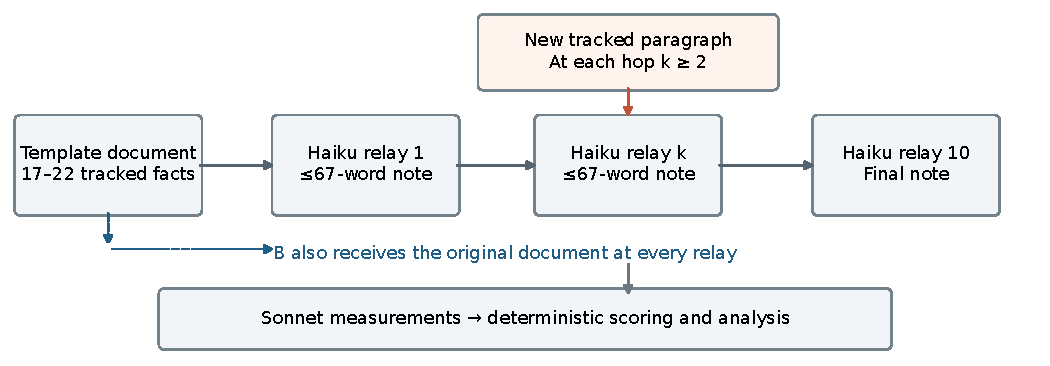
\includegraphics[width=\linewidth]{02_design.pdf}
  \caption{Data flow and measurement roles. Every relay produces a note. New paragraphs enter from
    hop 2; source access is the A/B manipulation. Measurement is separate from note
    generation. All relay requests sharing a batch nevertheless occupy one subagent context.}
  \label{fig:design}
\end{figure}

Implementation and orchestration were performed by the main Claude Code session. It
implemented the dataset builder, runner, batching, scoring and initial analysis, and
managed restarts after usage limits. Haiku subagents wrote the notes. Sonnet subagents
extracted answers and spans and judged semantic fact types. Step
agents ran orchestration commands and did not author experimental notes. Final aggregation
and optimization were deterministic Python computations.

\begin{table}[!htbp]
  \centering
  \small
  \caption{Measurement requests by role}
  \label{tab:measurement-roles}
  \begin{tabular}{@{}lr@{}}
    \toprule
    \textbf{Measurement role} & \textbf{Model requests} \\
    \midrule
    Extraction with spans & 24,003 \\
    Legacy extraction & 2,131 \\
    Judge under v2 rules & 11,893 \\
    Judge under strict m3 rules & 11,021 \\
    Invention audit & 9,680 \\
    \bottomrule
  \end{tabular}
\end{table}

The 58,728 measurement requests include checks and repeat extractions. Approximately 3,400
subagent launches and 35 million relay plus 290 million measurement tokens are
workflow estimates. The run used Claude Code subagents. The queue records the configured
aliases \path{subagent-haiku} and \path{subagent-sonnet}. Exact backend revisions remain
unverified.

\section{Retention and competition for the note}
\label{sec:retention}

At hop 10, original-fact kept counts are 440 and 73 in A-baseline and A-keep, and 1,179
and 1,305 in B-baseline and B-keep. Each cell has 4,674 fact observations. All 584,484
chain--hop--fact rows are present, with no duplicate keys. Paired document-bootstrap
estimates in Table~\ref{tab:endpoints} reproduce the original headline.

\begin{table}[!htbp]
  \centering
  \small
  \caption{Original fact correctness at hop 10 and paired document bootstrap intervals}
  \label{tab:endpoints}
  \begin{tabular}{@{}lrrrr@{}}
    \toprule
    \textbf{Cell} & \textbf{Baseline} & \textbf{Keep} & \textbf{Difference} & \textbf{95\% interval} \\
    \midrule
    A & $0.094138$ & $0.015618$ & $-0.078519$ & $[-0.085147,\,-0.071870]$ \\
    B & $0.252246$ & $0.279204$ & $+0.026958$ & $[+0.015142,\,+0.038785]$ \\
    \bottomrule
  \end{tabular}
\end{table}

In A, preservation initially helps originals by 7.17 percentage points at hop 1 and 6.95
at hop 2. The contrast becomes \ensuremath{-}5.50 points at hop 3, with a pointwise
interval of [\ensuremath{-}6.57, \ensuremath{-}4.47]. The notes at that crossover are
almost equal in length, 62.65 versus 62.32 words. Thus the reversal precedes the shorter
keep notes observed at the endpoint.

\begin{figure}[!htbp]
  \centering
  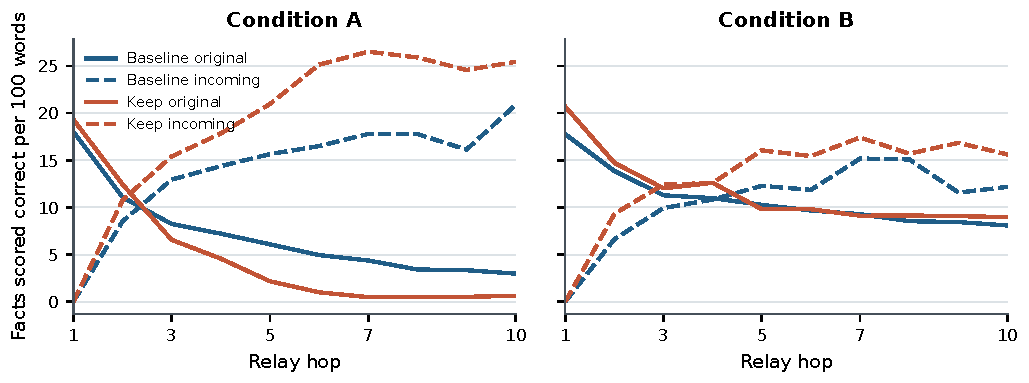
\includegraphics[width=\linewidth]{03_note_allocation.pdf}
  \caption{Note allocation measured as the mean within-note count of facts scored correct per 100
    whitespace-delimited words. Incoming counts cover all introduced cohorts. In A, the
    preservation arm shifts strongly toward incoming content; in B, both incoming and original
    densities can increase.}
  \label{fig:note-allocation}
\end{figure}

At hop 10 in A, original density falls from 2.98 to 0.62 facts per 100 words, while
incoming density rises from 20.88 to 25.45. The incoming-density difference is +4.56
[4.12, 5.02]. Original counts fall from 1.83 to 0.30 per note; incoming counts rise from
13.03 to 14.92. The newest cohort supplies 1.82 of the 1.89 additional incoming facts.
Total counted facts still increase slightly, from 14.86 to 15.22, so this is a change in
selection and packing rather than a fixed one-for-one substitution.

Keep also improves older incoming cohorts: after three relays their correctness is 0.186
rather than 0.098 in A. Recency therefore contributes to the endpoint pattern without
being a complete description of the prompt effect. These density measures depend on the
scoring system and count propositions of unequal word cost and importance.

One matched pair illustrates the allocation change at almost equal length. For
client\_request-x000, A, replicate 1, hop 10, the 60-word baseline begins ``Duneholm
Pharma: 336 GB supplier onboarding platform, go-live 26 April 2027.'' The 59-word keep
note begins ``Quince: coordinator Olwen Petrescu, 31 analysts, WS-BB20'' and contains only
workstream details. In this illustrative pair, the keep note scores zero original and
seventeen incoming facts, compared with two original and fourteen incoming facts under
baseline.

\section{Variation across documents and executions}
\label{sec:variation}

The A endpoint decrease appears in all four domains, from \ensuremath{-}6.75 to
\ensuremath{-}9.05 percentage points, and in 78 of 80 document-level comparisons. Dates
and numbers account for about 63\% of the aggregate decrease; names contribute another
18\%. Restricting to original facts labeled unguessable strengthens A's decrease to
\ensuremath{-}12.53 points. The direction therefore does not rely on guessable defaults.

\begin{figure}[!htbp]
  \centering
  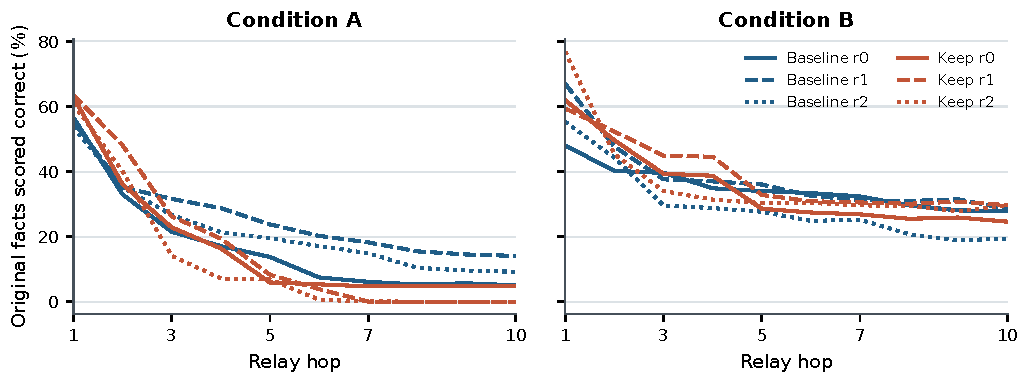
\includegraphics[width=\linewidth]{04_replicate_variation.pdf}
  \caption{Replicate trajectories reveal substantial execution variation. A-keep replicates 1 and 2
    contain zero original facts scored correct at hop 10 across all eighty documents. Distinct
    text outputs do not establish independence between requests answered in a shared context.}
  \label{fig:replicates}
\end{figure}

\begin{table}[!htbp]
  \centering
  \small
  \caption{Endpoint prompt effects by replicate in percentage points}
  \label{tab:replicates}
  \begin{tabular}{@{}lrrr@{}}
    \toprule
    \textbf{Endpoint effect in pp} & \textbf{Replicate 0} & \textbf{Replicate 1} & \textbf{Replicate 2} \\
    \midrule
    A keep minus baseline & $-0.32$ & $-14.06$ & $-9.18$ \\
    B keep minus baseline & $-3.21$ & $+1.16$ & $+10.14$ \\
    \bottomrule
  \end{tabular}
\end{table}

The B benefit is selective. Code retention rises from 0.204 to 0.533, while names,
negations and numbers decline. Excluding codes changes the B contrast to
\ensuremath{-}0.93 points [\ensuremath{-}2.08, +0.21]. This is a different estimand, but
it rules out describing the pooled increase as an improvement across fact types. Among
originals labeled guessable, B declines by 2.85 points; among those labeled unguessable,
it rises by 6.73.

Most relay batches contain forty requests from different documents within one condition,
arm and replicate. One subagent reads the batch and writes all responses. Avoiding
repeated documents limits direct leakage but does not remove common style, allocation
policy or context effects. At hop 10, one A-keep replicate-0 batch averages 1.825 original
facts; the other averages zero. The remaining A-keep endpoint batches are also uniformly
zero. The effective replication of subagent behavior is far smaller than the nominal fact
count.

Document-score correlations between B-baseline replicates range from \ensuremath{-}0.25 to
+0.62. A-keep correlations involving its all-zero replicates are undefined. A document
bootstrap preserves pairing but does not resample shared execution behavior. Multiway
dependence is therefore a design issue as well as an inferential
issue~\cite{cameronGelbachMiller2006}.

\section{Measurement error and factual correctness}
\label{sec:measurement}

Reference values and supporting source sentences are generated deterministically from
templates and fixed random seeds. This supplies exact reference facts by construction.
Measuring what remains in a compressed note also depends on the extractor, the semantic
judge, and the rubric for deciding whether the full fact is present.

Numbers, dates, names, codes, quantities and lists are classified deterministically from
Sonnet-extracted answers. Constraints, negations and conditionals also require Sonnet
judgments. Strict scoring adds span, unit, parameter and semantic-element checks.
Consequently, even deterministic status assignments depend on model-generated intermediate
answers.

\begin{figure}[!htbp]
  \centering
  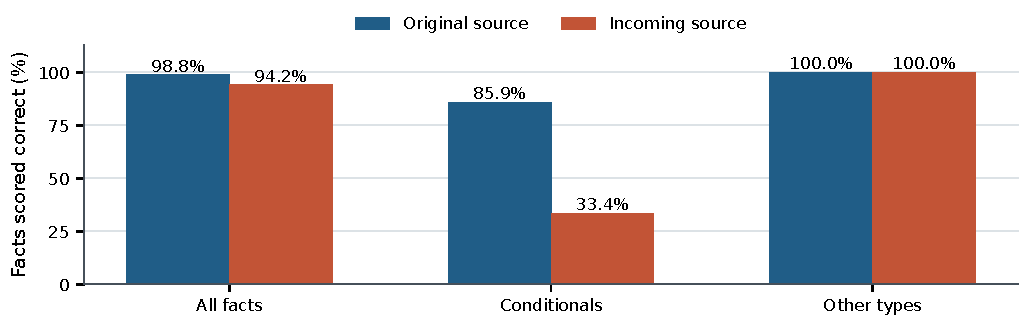
\includegraphics[width=\linewidth]{05_source_measurement.pdf}
  \caption{Source measurement exposes concentrated conditional-fact failures. Original source
    conditionals score 110/128 correct; incoming conditionals score 184/551. Every other fact
    type scores 100\% in the incoming own-paragraph check. The overall 94.2\% incoming rate
    conceals this concentration.}
  \label{fig:source-measurement}
\end{figure}

For example, a paragraph states that the Onyx trial repeats on 2027-10-29 if its score is
below 89. The extractor returns the repeat date without the threshold, and the strict
scorer marks the fact distorted. The underlying paragraph retained the full fact. Compact
notes can make the threshold easier to extract, creating apparent improvement without
restoration of information.

Let latent true retention be the fraction of fully retained facts. Let $\mathrm{Se}$ and
$\mathrm{Sp}$ denote the measurement sensitivity and specificity. Binary measured
correctness then satisfies

\begin{equation}
  \label{eq:measurement}
  R_{\mathrm{obs}}(t) = \mathrm{Se}(t) R_{\mathrm{true}}(t)
    + \bigl[1 - \mathrm{Sp}(t)\bigr]\bigl[1 - R_{\mathrm{true}}(t)\bigr].
\end{equation}

Estimating latent retention and differential measurement bias requires estimates of
these error rates by arm, type and note format. The spot check below provides only
limited coverage. Sensitivity measured on source passages may differ from sensitivity
on compressed notes. Retest agreement of 99.05\% falls to about 96.20\% where at least one
extraction is not missing. Stable errors can persist across repeats.

A copied span establishes textual occurrence. Entailment and role assignment require
separate checks. Heuristic recovery categories also require review. Plural ``engineers''
versus singular ``engineer'' can trigger an unsupported-value flag. The strong A decrease
nevertheless survives direct presence checks on unguessable names, codes and dates, making
a wholly judge-driven explanation implausible.

\subsection*{Human spot check of five notes}

The author completed the first five cases in the shuffled annotation packet and stopped
after those cases. The review presented each note and its reference claims with the arm,
hop and automated scores concealed. The author judged whether each full claim was present
in the note, then the labels were matched to the archived scores. The 93 judgments cover
original facts in five notes from five different documents. All notes are from condition A.

\begin{table}[!htbp]
  \centering
  \small
  \caption{Human judgments in the five-note spot check. Both archived scoring versions
    agreed with every label in these notes.}
  \label{tab:human-spot-check}
  \begin{tabular}{@{}llrrrrr@{}}
    \toprule
    \textbf{Hop} & \textbf{Arm} & \textbf{Notes} & \textbf{Facts}
      & \textbf{Kept} & \textbf{Distorted} & \textbf{Missing} \\
    \midrule
    3 & Baseline & 1 & 19 & 2 & 0 & 17 \\
    10 & Baseline & 3 & 56 & 4 & 1 & 51 \\
    10 & Keep & 1 & 18 & 1 & 0 & 17 \\
    \midrule
    & Total & 5 & 93 & 7 & 1 & 85 \\
    \bottomrule
  \end{tabular}
\end{table}

The author and both scoring versions agreed on 7 kept, 1 distorted and 85 missing facts
(Table~\ref{tab:human-spot-check}). The one distorted fact retained a 4\% late-delivery
penalty but omitted the requirement that delivery be more than ten days late and the
order value as the basis for the percentage. Agreement also left some room for interpretation.
For example, the reviewer and both scoring versions marked a requirement for 659
concurrent users as kept when the note specified 659 users without stating whether
they were concurrent.
The table reports the labels as recorded.

Most judgments were omissions, and the five notes contain no within-document pairs of
prompt arms. This limited coverage cannot establish a human-scored endpoint effect
or the reversal at hop 3. Estimating arm-specific error rates would require broader
coverage. The review covered only original facts in condition A and involved a single
reviewer. The primary results continue to use the archived automated scores.

\section{Mathematical models of retention}
\label{sec:models}

Let $Y$ be the indicator that a tracked fact is scored kept, and let $R(t)$ be its
marginal current-correctness probability after $t$ processing relays. For originals, $t$
equals the chain hop; incoming facts introduced at hop $j$ have age $t=k-j+1$ at calendar
hop $k$. Current correctness allows reappearance. Continuous survival instead requires a
fact to remain correct at every note since entry. The distinction matters most in B, where
the source is repeatedly available.

All four candidate curves multiply a normalized function by $R_0$. For original facts,
$R_0$ is fixed to measured source correctness, 0.988447 in the full dataset. For incoming
facts, source presentation is defined as one; only observed notes at ages 1--9 enter the
fit. No artificial age-zero rows are added.

\subsection*{Constant decay}

\begin{equation}
  \label{eq:constant}
  R(t) = R_0 p^t, \qquad 0 < p < 1.
\end{equation}

The survival interpretation assumes a common persistence probability and an absorbing loss
state. It implies a constant conditional loss hazard, 1 \ensuremath{-} p. Applied to
current correctness, it is a descriptive marginal restriction rather than a verified
transition mechanism.

\subsection*{A separate first relay}

\begin{equation}
  \label{eq:first-relay}
  R(t) = R_0 s p^{t-1} \quad (t \geq 1), \qquad R(0)=R_0.
\end{equation}

The initial inclusion parameter $s$ is separate from subsequent persistence $p$. For
incoming facts $s$ can exceed $p$: a newly presented paragraph is easy to include, but its
facts then face repeated competition. Calling this a first-hop loss shock would obscure
that direction.

\subsection*{Heterogeneous persistence}

\begin{equation}
  \label{eq:beta-geometric}
  p \sim \operatorname{Beta}(a,b), \qquad R(t) = R_0 \,\mathbb{E}[p^t]
    = R_0 \frac{\mathrm{B}(a+t,b)}{\mathrm{B}(a,b)}.
\end{equation}

This beta-geometric mixture~\cite{faderHardie2006} permits facts to differ in persistence
while each fact's latent $p$ remains fixed. Selection favors more persistent facts among
survivors. Under the absorbing-loss interpretation, the implied hazard is:

\begin{equation}
  \label{eq:beta-hazard}
  h(t) = 1 - \frac{R(t)}{R(t-1)} = \frac{b}{a+b+t-1}.
\end{equation}

\subsection*{A permanent component}

\begin{equation}
  \label{eq:cure}
  R(t) = R_0 \bigl[w + (1-w)q^t\bigr], \qquad 0 \leq w \leq 1.
\end{equation}

The cure family assigns a point mass $w$ to permanent survival and a geometric component
to the remainder~\cite{patileaVanKeilegom2017}. It is a model of a plateau-shaped curve.
Its permanent-survival interpretation requires assumptions that these ten-hop, measured
current-correctness data cannot verify.

\section{Estimation and predictive comparison}
\label{sec:estimation}

Parameters minimize the negative marginal Bernoulli log score, aggregated over actual
age-specific exposures. Write $x_t$ for kept counts and $n_t$ for the number of observed
facts at age $t$. We minimize $-\ell(\theta)$, where

\begin{equation}
  \label{eq:composite-likelihood}
  \ell(\theta) = \sum_{t=1}^{T} \left[
    x_t \log R_{\theta}(t) + (n_t-x_t)\log\bigl[1-R_{\theta}(t)\bigr]
  \right].
\end{equation}

This is a composite likelihood: repeated facts, chains and batch responses are dependent.
Constant decay has one fitted parameter; the other families have two. Optimization handles
the homogeneous boundary of the beta mixture and the zero-permanent-share boundary of
cure. Ordinary independent-binomial likelihood-ratio tests and their p-values are not
appropriate here.

Predictive comparison uses five folds split by whole documents, with source $R_0$
estimated from training documents in each fold. A fixed split seed of 20261109 makes the
comparison reproducible. Table~\ref{tab:predictive-comparison} reports held-out negative
log score per fact observation in nats; lower is better. These folds test other documents
within the recorded execution and can share batch behavior with training documents. They
are not a test of generalization to fresh subagent batches.

\begin{table}[!htbp]
  \centering
  \small
  \caption{Held out negative log scores per fact observation}
  \label{tab:predictive-comparison}
  \begin{tabular}{@{}lrrrr@{}}
    \toprule
    \textbf{Facts and cell} & \textbf{Constant} & \textbf{First relay} & \textbf{Beta mixture} & \textbf{Cure} \\
    \midrule
    Original A baseline & $0.49124$ & $0.47353$ & \textbf{0.47099} & $0.47264$ \\
    Original A keep & $0.30119$ & \textbf{0.30091} & $0.30119$ & $0.30114$ \\
    Original B baseline & $0.66857$ & $0.62617$ & \textbf{0.62375} & $0.62457$ \\
    Original B keep & $0.66021$ & $0.63347$ & $0.62891$ & \textbf{0.62813} \\
    Incoming A baseline & $0.33029$ & \textbf{0.31093} & $0.33029$ & $0.33029$ \\
    Incoming A keep & $0.38024$ & \textbf{0.33602} & $0.38024$ & $0.38024$ \\
    Incoming B baseline & $0.27395$ & \textbf{0.25489} & $0.27395$ & $0.27395$ \\
    Incoming B keep & $0.31978$ & \textbf{0.29989} & $0.31978$ & $0.31978$ \\
    \bottomrule
  \end{tabular}
\end{table}

The best family is beta-geometric for original A-baseline and B-baseline, first relay for
original A-keep and every incoming cell, and cure for original B-keep. Original A-keep
differences are small enough that the winner should not be treated as decisive.

Endpoint uncertainty uses 20,000 paired document resamples, keeping all cells and
replicates of a sampled document together. It therefore addresses document variation
conditional on these responses. An illustrative crossed document--replicate resampling
widens B's endpoint interval to [\ensuremath{-}3.26, +9.76] percentage points, but three
replicate blocks cannot calibrate a replacement execution-level interval.

For A-keep originals, first relay improves held-out log score over constant decay by only
0.00028 nats per observation; a document-resampled comparison interval includes zero. For
incoming facts, improvements are much larger, 0.019--0.044 nats. Their model ranking
persists under v2, uninterrupted survival, separate replicates and a balanced early-cohort
restriction.

\section{Models for original facts}
\label{sec:original}

\begin{figure}[!htbp]
  \centering
  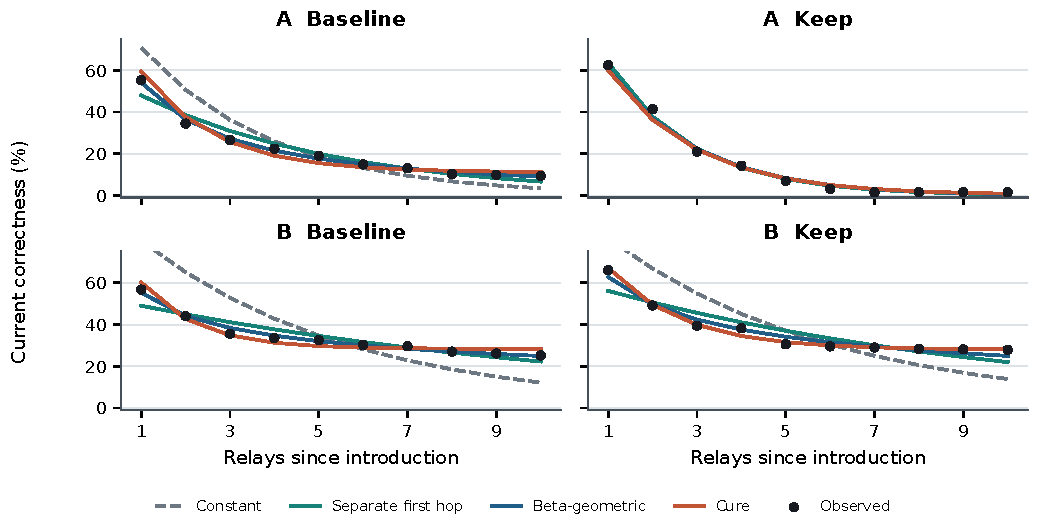
\includegraphics[width=\linewidth]{06_models_original.pdf}
  \caption{Original-fact curve fits. Black points are observed current correctness. Flexible families
    reproduce rapid early loss and slower tails more closely than a common constant rate,
    except in A-keep where the curves are close. These are marginal fits, not identified
    fact-level survival mechanisms.}
  \label{fig:original-fits}
\end{figure}

\begin{table}[!htbp]
  \centering
  \small
  \caption{Preferred original fact curves and fitted parameters}
  \label{tab:preferred-original-parameters}
  \begin{tabularx}{\linewidth}{@{}lXl@{}}
    \toprule
    \textbf{Cell} & \textbf{Preferred description} & \textbf{Fitted parameters} \\
    \midrule
    A baseline & Beta-geometric & $a = 1.407,\ b = 1.164$ \\
    A keep & First relay or near exponential & $s = 0.642,\ p = 0.595$ \\
    B baseline & Beta-geometric & $a = 0.466,\ b = 0.369$ \\
    B keep & Cure shaped & $w = 0.283,\ q = 0.551$ \\
    \bottomrule
  \end{tabularx}
\end{table}

A-baseline shows a pronounced first compression loss followed by deceleration. The beta
mixture captures that shape with a decreasing hazard. In a survival interpretation, facts
with weak persistence disappear early, enriching the remaining set for stronger facts. The
same aggregate shape can also arise from mixing fact types or batch-specific policies. A
marginal fit cannot identify stable persistence parameters for individual facts.

A-keep is approximately exponential over most of the observed decline, with a small late
remnant. Its beta fit reaches the homogeneous boundary, and its cure fit estimates a
normalized permanent share of only 0.0026. The extra first-relay parameter yields a small
predictive improvement. The data support rapid erosion, but do not decisively discriminate
these neighboring curves.

B-baseline favors a long, decelerating beta tail. Correctness still declines from 0.296 at
hop 7 to 0.252 at hop 10; a fixed plateau is premature. B-keep is more nearly flat late in
the window, and its cure-shaped fit approaches $R_0w \approx 0.280$. Because B can restore
omitted information from the source, that asymptote can describe repeated selection rather
than continuous survival.

Rankings depend on composition and execution: cure becomes nominally best in both
unguessable baseline subsets, and B-keep replicates disagree about the preferred family.

\section{Models for incoming cohorts}
\label{sec:incoming}

\begin{figure}[!htbp]
  \centering
  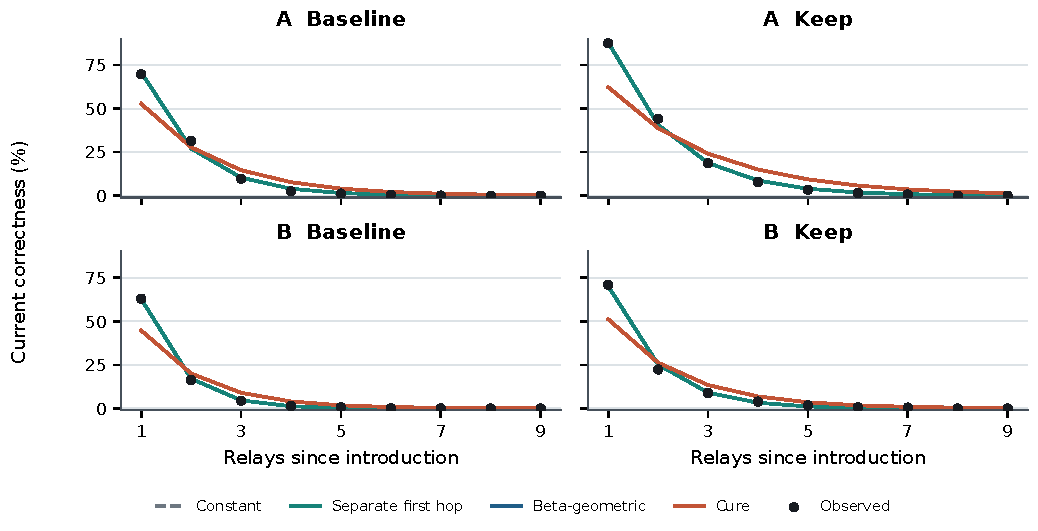
\includegraphics[width=\linewidth]{07_models_incoming.pdf}
  \caption{Incoming-fact fits by relay age. A high initial inclusion probability followed by
    substantially poorer persistence requires a separate first relay. Standard beta-geometric
    and cure families cannot represent the rise in loss hazard after the first relay and move to nearly
    homogeneous or zero-cure boundaries.}
  \label{fig:incoming-fits}
\end{figure}

\begin{table}[!htbp]
  \centering
  \small
  \caption{Incoming first relay parameters and integrated fitted curves}
  \label{tab:incoming-parameters}
  \begin{tabular}{@{}lrrr@{}}
    \toprule
    \textbf{Cell} & \textbf{Initial inclusion $s$} & \textbf{Later persistence $p$} & \textbf{Curve area $s/(1-p)$} \\
    \midrule
    A baseline & $0.707$ & $0.383$ & $1.15$ \\
    A keep & $0.879$ & $0.462$ & $1.64$ \\
    B baseline & $0.628$ & $0.272$ & $0.86$ \\
    B keep & $0.702$ & $0.359$ & $1.10$ \\
    \bottomrule
  \end{tabular}
\end{table}

In A-baseline, the fitted initial loss probability is 0.293, followed by a later loss
probability of 0.617. Under keep, these become 0.121 and 0.538. Preservation therefore
improves both admission and subsequent persistence of incoming facts, although later loss
remains severe. The B cells exhibit the same asymmetry with lower incoming persistence,
consistent with competition from the repeatedly available original source.

The initial parameters are fitted to all cohorts, not simply copied from the first
observed paragraph. The mean observed one-relay incoming correctness is 0.697 versus 0.875
in A, and 0.630 versus 0.709 in B. Differences from fitted $s$ reflect the joint fit to
later ages and their exposure weights.

Summing the fitted curve over all future ages gives $s/(1-p)$, shown in the last column.
Under an absorbing, stationary interpretation it is the expected number of correct note
appearances per introduced fact, including facts never admitted. It is a model
extrapolation rather than an observed lifetime or a calibrated memory capacity.
Current-correctness noise and reappearance further weaken a literal survival reading.

Pooling by age changes cohort composition: only the earliest cohort reaches age nine. The
next section tests whether an age-averaged curve reconstructs incoming counts at each
calendar hop.

\section{Cohort convolution and stationarity}
\label{sec:stationarity}

An age curve describes the fate of one cohort. A note at calendar hop $k$ contains a
mixture of cohorts. Let $m_j$ be the mean number of facts introduced at hop $j$ and $C(k)$
the expected incoming count in a note. A stationary age model implies the cohort
convolution:

\begin{equation}
  \label{eq:cohort-convolution}
  C(k) = \sum_{j=2}^{k} m_j R(k-j+1).
\end{equation}

For a constant incoming cohort size $m$ and the separate-first-relay model, the finite sum
and its limiting value have closed forms:

\begin{equation}
  \label{eq:cohort-limit}
  C(k) = ms \frac{1-p^{k-1}}{1-p}, \qquad C_{\infty} = \frac{ms}{1-p}.
\end{equation}

\begin{figure}[!htbp]
  \centering
  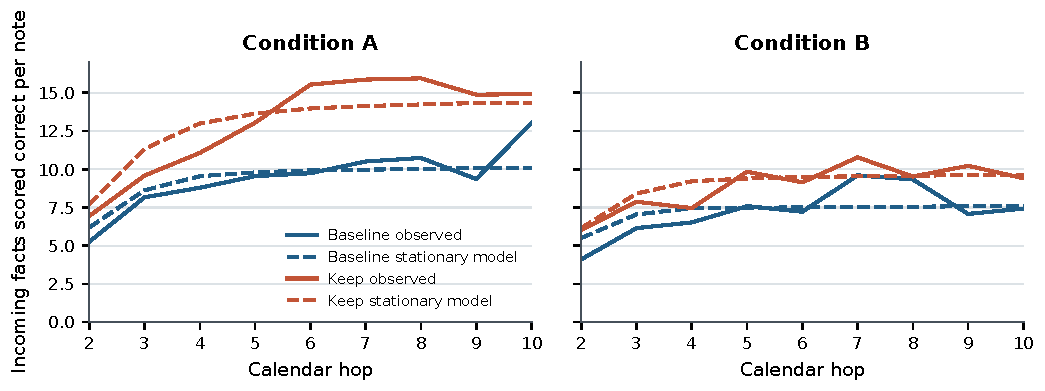
\includegraphics[width=0.95\linewidth]{08_cohort_occupancy.pdf}
  \caption{Observed incoming counts and counts predicted by convolving actual cohort sizes with the
    fitted age curve. Dashed lines are not refitted to calendar-hop totals. A-baseline shows a
    marked failure of the stationary approximation, despite the first-relay model being its
    best candidate age curve.}
  \label{fig:cohort-occupancy}
\end{figure}

\begin{table}[!htbp]
  \centering
  \small
  \caption{Incoming counts at hop 10. Differences use unrounded values.}
  \label{tab:cohort-predictions}
  \begin{tabular}{@{}lrrr@{}}
    \toprule
    \textbf{Cell at hop 10} & \textbf{Observed} & \textbf{Age-model prediction} & \textbf{Observed minus predicted} \\
    \midrule
    A baseline & $13.03$ & $10.07$ & $+2.95$ \\
    A keep & $14.92$ & $14.35$ & $+0.56$ \\
    B baseline & $7.43$ & $7.58$ & -0.15 \\
    B keep & $9.41$ & $9.63$ & -0.21 \\
    \bottomrule
  \end{tabular}
\end{table}

The stationary calculation predicts 10.07 incoming facts at A-baseline hop 10, compared
with 13.03 observed. It is much closer in the other cells: 14.35 versus 14.92 in A-keep,
7.58 versus 7.43 in B-baseline and 9.63 versus 9.41 in B-keep. These discrepancies are
descriptive diagnostics, not a formal goodness-of-fit test with independent observations.

A good age-averaged curve can therefore fail to reconstruct the changing allocation of a
note. Admission or persistence may depend on calendar hop, the amount of surviving
original content, cohort wording, or shared subagent behavior. Models with a birth-cohort
inclusion parameter and calendar-dependent transition rates are plausible next candidates,
but their extra flexibility should be judged on independent execution blocks and later
held-out hops.

\section{Plateaus, recovery, and long-horizon identification}
\label{sec:identification}

A plateau-shaped current-correctness curve does not uniquely identify permanent survival.
In a homogeneous two-state process with loss probability $e$ and recovery probability $r$,
the recurrence and its solution are:

\begin{equation}
  \label{eq:recovery-recurrence}
  R(t+1) = (1-e)R(t) + r\bigl[1-R(t)\bigr].
\end{equation}

\begin{equation}
  \label{eq:recovery-solution}
  R(t) = \pi + (R_0-\pi)(1-e-r)^t, \qquad \pi = \frac{r}{e+r}.
\end{equation}

This has the same form as the cure curve when $\pi=R_0w$ and $q=1-e-r$. Thus marginal
curve fit cannot distinguish a permanent subset from loss and recovery. Transition counts
help only when measured states, homogeneous rates and their time stability are credible.
Source access, shared contexts and extraction errors complicate all three assumptions.

\begin{figure}[!htbp]
  \centering
  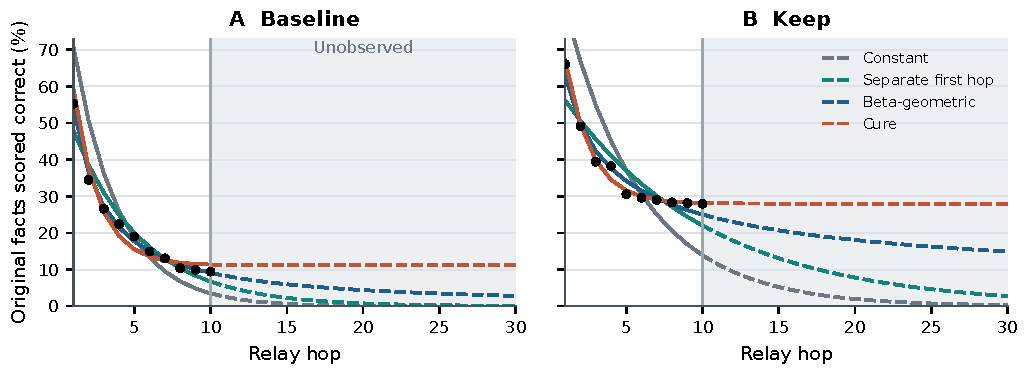
\includegraphics[width=\linewidth]{09_extrapolation.pdf}
  \caption{Models fitted through hop 10 diverge beyond the observation window. The shaded region
    contains predictions, not experimental data. A-baseline illustrates disagreement about
    eventual decline versus a positive plateau; B-keep illustrates how similar short-window
    fits can support different long-run interpretations.}
  \label{fig:extrapolation}
\end{figure}

The beta mixture supplies a second warning. Its normalized tail behaves as a power law:

\begin{equation}
  \label{eq:beta-tail}
  \frac{R(t)}{R_0} \sim \frac{\Gamma(a+b)}{\Gamma(a)}\, t^{-b},\qquad t\to\infty.
\end{equation}

For $b\leq 1$, the formal mean first-loss time diverges even though the permanent share is
zero. B-baseline's fitted $b\approx 0.369$ falls in that range. This is a property of an
unverified extrapolation, not evidence of infinite model memory. Ten hops do not identify
the tail. Even tight conditional bootstrap intervals on $w$ omit structural uncertainty
and fresh-execution variation.

Uninterrupted survival is lower than endpoint current correctness, especially in B:
approximately 0.222 versus 0.252 for baseline and 0.240 versus 0.279 for keep. No
observation beyond hop 10 is available in this run. A longer apparent plateau would
strengthen a finite-horizon forecast but could never prove literal permanent retention.

\section{Interpretation and next experiments}
\label{sec:interpretation}

The results support a narrow conclusion: in this batched subagent execution, a generic
instruction to preserve specifics changes which facts occupy a short note. Without source
access, an early advantage for original facts reverses by hop 3, while incoming details
become denser. With source access, the pooled endpoint gain is smaller and concentrated in
codes. The arithmetic is well reproduced; the model-level generality and the causal
mechanism are less secure.

Length alone is inadequate. A-keep is about four words shorter at hop 10, yet the negative
original contrast remains after excluding over-budget notes and within a common
58--67-word range. Incoming density gains also survive character-based denominators. Those
checks are descriptive because length is affected by the prompt. A whitespace word budget
is not a constant token or information budget, and the requested limit was sometimes
exceeded.

Recency and prose structure remain plausible contributors. New paragraphs are always
appended and explicitly labeled new; preservation is instructed after them. They are not
denser in tracked facts per input word than originals, approximately 8.76 versus 9.78 per
100 words, but their recurring anchors may facilitate compact lists. Prior
position-sensitivity findings motivate order controls~\cite{liuEtAl2024}. The mechanism in
these much shorter summaries remains open.

\subsection*{Three experiments with the highest information value}

First, isolate execution. Compare one request per fresh subagent context against the
current batching protocol, randomize order and document grouping, record exact
served-model metadata, and obtain enough independent execution blocks to estimate
variability. This directly tests whether the reversal and the B benefit replicate outside
shared-context response generation.

Second, manipulate capacity and interference with matched facts. Cross baseline and keep
with larger budgets and zero or current incoming load, controlling paragraph length with
filler where needed. Counterbalance equivalent facts between original and incoming roles,
their order and workstream phrasing. A capacity account predicts attenuation when space
expands or new fact load disappears.

Third, freeze model forecasts and extend independent chains to at least 30--50 hops.
Randomize whether incoming information continues or stops at a preregistered hop,
retaining the A/B distinction. Score both current correctness and uninterrupted survival
by cohort. This tests extrapolation and the contribution of continual interference without
equating a fitted asymptote with permanence.

\subsection*{Further human validation}

A follow-up audit should use two independent reviewers and matched notes from both
prompt arms for each sampled document and hop. Reviewers should check reference-to-question
alignment and judge the notes directly, attending to extraction fidelity, role, units,
scope, condition, threshold and consequence. Coverage of incoming facts would test whether
the change in composition is visible to human readers. Separate diagnostic samples can
target source conditionals, recoveries and scoring disagreements. The analysis should
account for clustered judgments, stratified sampling and sparse retained outcomes. For B's
2.70-point effect, uncertainty about differential measurement bias would need to be
materially smaller than the effect.

\FloatBarrier
\appendix

\section{Technical appendix}

\subsection*{Original curve parameters under all four families}

\begin{table}[!htbp]
  \centering
  \small
  \caption{Original fact parameters for all candidate models}
  \label{tab:original-parameters}
  \begin{tabular}{@{}lrrrr@{}}
    \toprule
    \textbf{Cell} & \textbf{Constant $p$} & \textbf{First relay $(s,p)$} & \textbf{Beta $(a,b)$} & \textbf{Cure $(w,q)$} \\
    \midrule
    A baseline & $0.7154$ & $0.4847,\ 0.8037$ & $1.4068,\ 1.1643$ & $0.1126,\ 0.5491$ \\
    A keep & $0.6093$ & $0.6422,\ 0.5945$ & Homogeneous limit & $0.0026,\ 0.6041$ \\
    B baseline & $0.8112$ & $0.4960,\ 0.9162$ & $0.4665,\ 0.3688$ & $0.2872,\ 0.4504$ \\
    B keep & $0.8218$ & $0.5678,\ 0.9012$ & $0.8507,\ 0.4892$ & $0.2832,\ 0.5507$ \\
    \bottomrule
  \end{tabular}
\end{table}

All original curves use $R_0=0.988447$. The homogeneous beta boundary is numerical: mean
persistence remains finite while concentration increases, recovering constant decay. It is
not evidence for substantive heterogeneity parameters of enormous magnitude. Every
incoming beta fit approaches the same boundary, and every incoming cure fit reaches its
numerical zero-share boundary.

\subsection*{Conditional uncertainty of the permanent component}

\begin{table}[!htbp]
  \centering
  \small
  \caption{Conditional document bootstrap intervals for the cure parameter}
  \label{tab:cure-intervals}
  \begin{tabular}{@{}lrr@{}}
    \toprule
    \textbf{Cell} & \textbf{Fitted $w$} & \textbf{Document bootstrap 95\% interval} \\
    \midrule
    A baseline & $0.1126$ & $[0.1053,\,0.1194]$ \\
    A keep & $0.0026$ & $[0.0000,\,0.0063]$ \\
    B baseline & $0.2872$ & $[0.2750,\,0.2979]$ \\
    B keep & $0.2832$ & $[0.2717,\,0.2951]$ \\
    \bottomrule
  \end{tabular}
\end{table}

These 400-draw parameter intervals hold the empirical source floor fixed and condition on
the selected cure family and recorded measurements. They are not intervals for a
demonstrated never-lost share. Their narrowness does not resolve model misspecification,
measurement bias, batch dependence or finite-horizon identification.

\subsection*{Survivor selection in the beta mixture}

Under absorbing loss and a fixed latent persistence probability, observing survival
through $t$ relays multiplies the beta prior density by $p^t$. The survivor distribution
is therefore $\operatorname{Beta}(a+t,b)$. Its expected next-step persistence is
$(a+t)/(a+b+t)$, which yields the decreasing hazard in \eqref{eq:beta-hazard}. The
deceleration is a compositional effect: individual facts need not improve with age. This
derivation concerns true survival; using it for current measured correctness requires the
additional assumptions discussed above.

\subsection*{Checks on alternative endpoints and composition}

Under v2, endpoint keep-minus-baseline differences are \ensuremath{-}7.895 points in A and
+2.589 in B, compared with \ensuremath{-}7.852 and +2.696 under strict m3. Literal value
presence among unguessable original names, codes and full dates falls from 0.162 to 0.021
in A and rises from 0.409 to 0.535 in B. Neither check validates role assignment. Small
numeric values may occur in unrelated dates or codes, so analogous number-presence checks
are less informative.

All incoming facts are labeled unguessable, versus 57.9\% of original facts. These are
generator-defined categories. The five-note audit checked retention and did not test how
often people can reconstruct facts from context.

\FloatBarrier
\section*{Reproducibility}

\addcontentsline{toc}{section}{Reproducibility}

\subsection*{Data and computational record}

The accompanying repository provides scored fact rows and an offline script that
recomputes the four original-fact correctness rates at hop 10 and regenerates
Figure~\ref{fig:original-retention}. Its README identifies the inputs and documents
the command. This check starts from the archived score labels. Running the relay and
scoring pipeline again would require the original execution setup.

The wider local archive includes synthetic source documents, relay notes, queue records,
and the annotation records for the five-note human spot check. The archived scores and
notes have SHA-256 prefixes \path{ff91a0d6f0fbcece372a9dba3aadc5f9}
and \path{41e24d0d9e3fdc81dd9bb19f72814fe1}, respectively. The local analysis used Python 3.12.13,
NumPy 2.5.4, pandas 3.1.0, SciPy 1.18.1 and Matplotlib 3.11.2. The curve extrapolations
are labeled as predictions in the figures.

\subsection*{Execution accounting}

Stored manifests contain 240 relay batches covering 9,590 analyzed responses. Most batches
contain forty requests; one contains thirty. Ten initial test responses complete the total
of 9,600 notes. This accounting reconciles the initial test with the nominal forty-request
batch protocol rather than adding it to 240 complete forty-request batches. Launch totals
of roughly 250 for relay and 3,100 for measurement include orchestration agents and are
approximate.

\subsection*{Scope of the evidence}

The article concerns the 80-document, ten-hop run. Earlier exploratory runs used different
incoming-prose generation and cannot isolate the reason for a cross-study reversal. The
automated measurements and the five-note human spot check come from the same batched
execution. Generalization to fresh contexts and to longer chains remains open. The
preservation prompt changed measured content selection under this compression, input and
harness configuration.

\FloatBarrier
\bibliographystyle{unsrtnat}
\bibliography{references}

\end{document}
